\section{Model}

\subsection{Dynamika serwa}

Dynamikę serwomechanizmu w pierwszym przybliżeniu opisuje się jako człon
inercyjny I rzędu:
\begin{equation}
  G_{\mathrm{serwo}}(s)=\frac{1}{Ts+1},
\end{equation}
gdzie $T$ jest stałą czasową (im mniejsza wartość $T$, tym szybsza odpowiedź na
skok sygnału sterującego).

Transmitancja serwa $G_{\mathrm{serwo}}(s)$ jest stosunkiem transformaty Laplace'a 
kąta serwa $\Theta_{\mathrm{serwo}}(s)$ do transformaty Laplace'a sygnału wejściowego 
(napięcia sterującego) $U(s)$ w dziedzinie Laplace'a:
\begin{equation}
  G_{\mathrm{serwo}}(s) = \frac{\Theta_{\mathrm{serwo}}(s)}{U(s)}
\end{equation}

W kartach katalogowych serwomechanizmów podawana jest zwykle prędkość typu
„$t\,\mathrm{s}/60^{\circ}$”, która opisuje maksymalną szybkość przestawiania
(\emph{slew rate}), a nie bezpośrednio stałą czasową $T$. W modelu uproszczonym
przyjmuje się jednak, że wraz ze wzrostem prędkości katalogowej maleje efektywna
stała czasowa.

W nocie katalogowe do serwa podano predkosci przy róznych napieciach zasilania:
\begin{itemize}
  \item $0{,}20\,\mathrm{s}/60^{\circ}$ przy $4{,}8\,\mathrm{V}$,
  \item $0{,}11\,\mathrm{s}/60^{\circ}$ przy $6\,\mathrm{V}$.
\end{itemize}


Przy napięciu $5\,\mathrm{V}$, 
prędkość wyniesie około:
\begin{equation}
V_{5V}\approx 0{,}20 - \left(\frac{0{,}09}{1{,}2} \cdot 0{,}2\right) \approx 0{,}185\,\mathrm{s}/60^{\circ}
\end{equation}

Jeśli serwo potrzebuje $0{,}185\,\mathrm{s}$ na pokonanie $60^{\circ}$, to jego 
prędkość maksymalna wynosi ok. $324^{\circ}/\mathrm{s}$.

W klasycznym modelu $G(s)=\frac{1}{Ts+1}$, czas odpowiedzi (10\%--90\%) wynosi 
ok. $2{,}2T$. Jeśli założymy, że dla małych skoków dynamika jest zbliżona do czasu 
przemieszczenia podanego w specyfikacji. Dla
$6\,\mathrm{V}$($0{,}11\,\mathrm{s}/60^{\circ}$) $T$ mogłoby wynosić ok
$\mathrm{V}$$0{,}05$--$0{,}07\,\mathrm{s}$. Więc dla $5\,\mathrm{V}$
($0{,}185\,\mathrm{s}/60^{\circ}$) $T$ może wynosić $0{,}095\,\mathrm{s}$ .

Ostatecznie dynamika serwa bedzie opisana jako:

\begin{equation}
  G_{\mathrm{serwo}}(s)=\frac{\Theta_{\mathrm{serwo}}(s)}{U(s)}=\frac{1}{T_{\mathrm{serwo}}s+1},
\end{equation}


\subsection{Dynamika piłeczki na belce}

Rozpatrując dynamikę piłeczki na belce, wyprowadzamy równanie wiążące kąt belki 
($\theta$) z przyspieszeniem liniowym piłeczki ($\ddot{x}$). 

\subsubsection{II Zasada Dynamiki $F=ma$}

\begin{figure}[H]
  \centering
  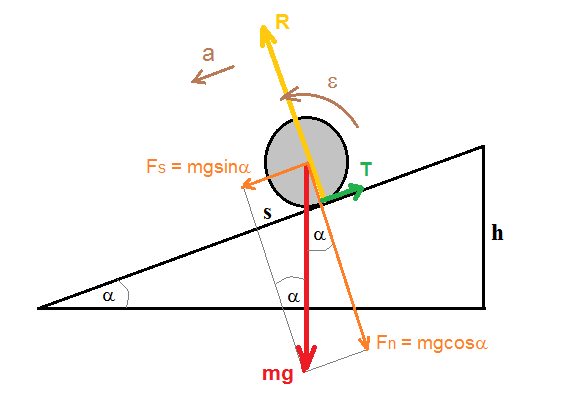
\includegraphics[width=0.5\linewidth]{source/2-model/2-model-img/silybelka.png}
  \caption{Rozkład sił działajacych na kule na równi pochyłej}
\end{figure}

Patrzmy na siły działające wzdłuż belki:
\begin{itemize}
  \item Grawitacja ($F_g$): Jej składowa równoległa do belki wynosi $m \cdot g \cdot \sin(\theta)$.
  \item Tarcie ($T$): Działa w górę belki i zmusza piłeczkę do obrotu.
\end{itemize}

Równanie Newtona dla ruchu postępowego:
\begin{equation}
m \cdot \ddot{x} = m \cdot g \cdot \sin(\theta) - T
\end{equation}

\subsubsection{II Zasada Dynamiki $M=J\epsilon$}

Moment obrotowy wokół własnej osi piłeczki jest generowany przez siłę tarcia na 
ramieniu promienia $R$(promień piłeczki):
\begin{equation}
T \cdot R = J \cdot \ddot{\alpha}
\end{equation}
gdzie $J$ to moment bezwładności piłeczki, a $\ddot{\alpha}$ to przyspieszenie kątowe.

\subsubsection{Warunek Toczenia bez Poślizgu}

Piłeczka toczy się bez poślizgu, co oznacza, że przyspieszenie liniowe zależy od 
przyspieszenia kątowego:
\begin{equation}
\ddot{x} = \ddot{\alpha} \cdot R \quad \Rightarrow \quad \ddot{\alpha} = \frac{\ddot{x}}{R}
\end{equation}

\subsubsection{Eliminacja Tarcia i Przyspieszenia Kątowego}

Z warunku toczenia bez poślizgu podstawiamy $\ddot{\alpha}$ do równania momentu:
\begin{equation}
T \cdot R = J \cdot \frac{\ddot{x}}{R} \quad \Rightarrow \quad T = \frac{J \cdot \ddot{x}}{R^2}
\end{equation}

Teraz wstawiamy to wyrażenie na $T$ do równania ruchu postępowego:
\begin{equation}
m \cdot \ddot{x} = m \cdot g \cdot \sin(\theta) - \frac{J \cdot \ddot{x}}{R^2}
\end{equation}

\subsubsection{Rozwiązanie dla Przyspieszenia Liniowego}

Przenosimy człon z $\ddot{x}$ na lewą stronę:
\begin{equation}
m \cdot \ddot{x} + \frac{J \cdot \ddot{x}}{R^2} = m \cdot g \cdot \sin(\theta)
\end{equation}

Wyciągamy $\ddot{x}$ przed nawias:
\begin{equation}
\ddot{x} \left( m + \frac{J}{R^2} \right) = m \cdot g \cdot \sin(\theta)
\end{equation}

Dzielimy przez nawias:
\begin{equation}
\ddot{x} = \frac{m \cdot g \cdot \sin(\theta)}{m + \frac{J}{R^2}}
\end{equation}

Dzieląc licznik i mianownik przez masę $m$:
\begin{equation}
\ddot{x} = \frac{g \cdot \sin(\theta)}{1 + \frac{J}{m R^2}}
\end{equation}

Dla małych kątów $\sin(\theta) \approx \theta$, ostatecznie otrzymujemy:
\begin{equation}
\ddot{x} = \frac{g}{1 + \frac{J}{m R^2}} \cdot \theta
\end{equation}
gdzie współczynnik:
\begin{equation}
\frac{g}{1 + \frac{J}{m R^2}}=c_{\mathrm{ball}}
\end{equation}
ostatecznie:
\begin{equation}
\ddot{x}=c_{\mathrm{ball}} \cdot \theta
\end{equation}

\subsubsection{Paramter $c_{\mathrm{ball}}$}

\begin{equation}
c_{\mathrm{ball}} = \frac{g}{1 + \frac{J}{m R^2}}
\end{equation}


Moment bezwładności: $J = \frac{2}{3} m R^2$. 
Podstawiając do mianownika:
\begin{equation}
1 + \frac{\frac{2}{3} m R^2}{m R^2} = 1 + \frac{2}{3} = \frac{5}{3} \approx 1{,}667
\end{equation}

Współczynnik:
\begin{equation}
c_{\mathrm{ball}} = \frac{g}{1{,}667} = \frac{3}{5} g = 0{,}6 \, g
\end{equation}

Stała $c_{\mathrm{ball}}$ wyznaczająca dynamikę piłeczki wynosi:
\begin{equation}
c_{\mathrm{ball}} = 0{,}6 \cdot 9{,}81 = 5{,}886 \, \mathrm{m/s^2}
\end{equation}

\subsubsection{Transmitancja piłeczki na belce}

Równanie dynamiki piłeczki w dziedzinie czasu jest następujące:
\begin{equation}
\ddot{x}=c_{\mathrm{ball}} \cdot \theta
\end{equation}

Stosujemy transformatę Laplace'a. Dla warunków początkowych ($x(0) = 0$, $\dot{x}(0) = 0$, $\theta(0) = 0$):
\begin{equation}
\mathcal{L}\{\ddot{x}(t)\} = s^2 \cdot X(s)
\end{equation}
\begin{equation}
\mathcal{L}\{\theta(t)\} = \Theta(s)
\end{equation}

\begin{equation}
s^2 \cdot X(s) = c_{\mathrm{ball}} \cdot \Theta(s)
\end{equation}

\paragraph{Wyznaczenie Transmitancji:}

Transmitancja jest definiowana jako stosunek transformaty Laplace'a wyjścia do 
transformaty Laplace'a wejścia (przy zerowych warunkach początkowych):
\begin{equation}
G_{\mathrm{ball}}(s) = \frac{X(s)}{\Theta_{\mathrm{beam}}(s)}=\frac{c_{\mathrm{ball}}}{s^2}
\end{equation}

\subsection{Transmitancja całego układu}

Posiadając kompletny zestaw opisu dynamik elementów układu, możemy teraz połączyć 
transmitancję serwa z transmitancją piłeczki na belce, uwzględniając mechaniczne 
połączenie między nimi.

\subsubsection{Zależnośc pomiedzy $\Theta_{serwo}$ i $\Theta_{beam}$}

\begin{figure}[H]
  \centering
  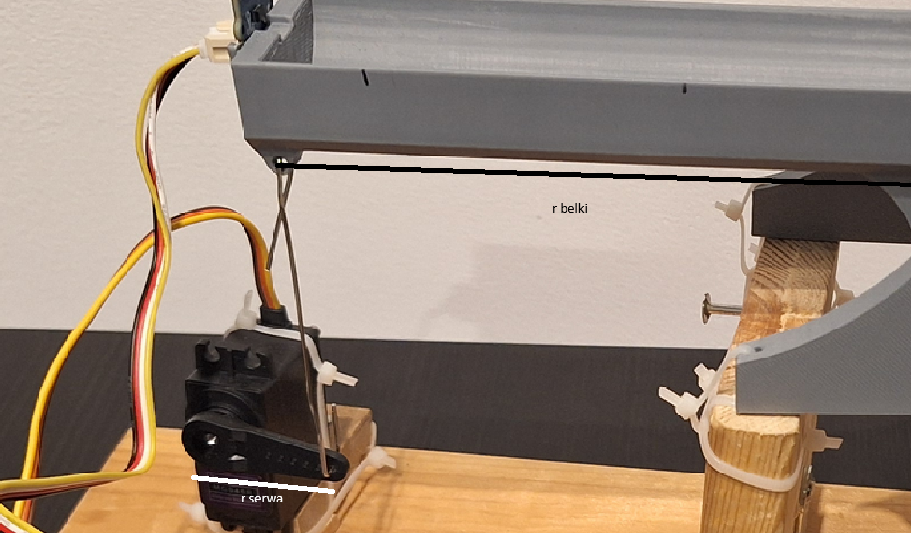
\includegraphics[width=0.5\linewidth]{source/2-model/2-model-img/kmech.png}
  \caption{fizyczne mechaniczne połączenie pomiedzy serwem i belką}
\end{figure}
 
Zakładając idealne połączenie pomiedzy serwem i belką, obowiązuje 
następująca zależność kinematyczna:

\begin{equation}
r_{\mathrm{serwo}} \cdot \theta_{\mathrm{serwo}} = r_{\mathrm{belka}} \cdot \theta_{\mathrm{belka}}
\end{equation}

gdzie:
\begin{itemize}
  \item $r_{\mathrm{serwo}}$ -- promień dźwigni na wale serwa($3\,\mathrm{cm}$),
  \item $r_{\mathrm{belka}}$ -- promień dźwigni na wale belki($15\,\mathrm{cm}$),
\end{itemize}

Stąd wynika relacja kątów:

\begin{equation}
\theta_{\mathrm{belka}} = \frac{r_{\mathrm{serwo}}}{r_{\mathrm{belka}}} \cdot \theta_{\mathrm{serwo}} = k_{mech} \cdot \theta_{\mathrm{serwo}}
\end{equation}

Gdzie $k_{mech}$ jest przekładnią mechaniczna.

\subsubsection{Połączenie Szeregowe Transmitancji}

Układ składa się z dwóch elementów połączonych szeregowo:
\begin{itemize}
  \item Serwo: $G_{\mathrm{serwo}}(s) = \frac{\Theta_{\mathrm{serwo}}(s)}{U(s)} = \frac{1}{T_{\mathrm{serwo}} s + 1}$
  \item Piłeczka na belce: $G_{\mathrm{ball}}(s) = \frac{X(s)}{\Theta_{\mathrm{belka}}(s)} = \frac{c_{\mathrm{ball}}}{s^2}$
\end{itemize}

Dla połączenia szeregowego bez sprzężeń zwrotnych, ścieżka sygnału przebiega:

\begin{equation}
U(s) \xrightarrow{G_{\mathrm{serwo}}} \Theta_{\mathrm{serwo}}(s) \xrightarrow{k_{mech}} \Theta_{\mathrm{belka}}(s) \xrightarrow{G_{\mathrm{ball}}} X(s)
\end{equation}

Transmitancja piłeczki wynosi:
\begin{equation}
G_{\mathrm{ball}}(s) = \frac{X(s)}{\Theta_{\mathrm{belka}}(s)}
\end{equation}

 Musimy podstawić 
relację $\Theta_{\mathrm{belka}}(s) = k_{\mathrm{mech}} \cdot \Theta_{\mathrm{serwo}}(s)$:

\begin{equation}
G_{\mathrm{ball}}(s) = \frac{X(s)}{\Theta_{\mathrm{belka}}(s)} = \frac{X(s)}{k_{\mathrm{mech}} \cdot \Theta_{\mathrm{serwo}}(s)} 
\end{equation}

Stąd wynika:
\begin{equation}
X(s) = k_{\mathrm{mech}h} \cdot G_{\mathrm{ball}}(s) \cdot \Theta_{\mathrm{serwo}}(s)
\end{equation}

Teraz, znając że $\Theta_{\mathrm{serwo}}(s) = G_{\mathrm{serwo}}(s) \cdot U(s)$, mamy:

\begin{equation}
X(s) = k_{\mathrm{mech}} \cdot G_{\mathrm{ball}}(s) \cdot G_{\mathrm{serwo}}(s) \cdot U(s)
\end{equation}

Stąd transmitancja całkowita:

\begin{equation}
G_{\mathrm{total}}(s) = \frac{X(s)}{U(s)} = k_{\mathrm{mech}} \cdot G_{\mathrm{ball}}(s) \cdot G_{\mathrm{serwo}}(s)
\end{equation}

Podstawiając transmitancje:

\begin{equation}
G_{\mathrm{total}}(s) = k_{\mathrm{mech}} \cdot \frac{c_{\mathrm{ball}}}{s^2} \cdot \frac{1}{T_{\mathrm{serwo}} s + 1}
\end{equation}

\subsubsection{Ostateczna Forma Transmitancji Całego Układu}

\begin{equation}
G_{\mathrm{total}}(s) =\frac{k_{\mathrm{mech}} \cdot c_{\mathrm{ball}}}{s^2 \cdot (T_{\mathrm{serwo}} s + 1)}
\end{equation}

Rozwijając mianownik:

\begin{equation}
G_{\mathrm{total}}(s) = \frac{k_{\mathrm{mech}} \cdot c_{\mathrm{ball}}}{T_{\mathrm{serwo}} s^3 + s^2}
\end{equation}

Gdzie:
\begin{itemize}
  \item $k_{\mathrm{mech}}=\frac{3cm}{15cm}=0,2$
  \item $c_{\mathrm{ball}}=5,586$
  \item $T_{\mathrm{serwo}}=0.095$
\end{itemize}








